
% !TEX encoding = UTF-8 Unicode 
% !TEX root = FieldGuide.tex

\Sec{Beta-Exponential Distribution}
\label{sec:BetaExp}

\phantomsection
\addcontentsline{toc}{subsection}{~~~~~~~~~~~~Beta-exponential}
\phantomsection
\addcontentsline{toc}{subsection}{~~~~~~~~~~~~Standard beta-exponential}
The {\bf beta-exponential} (Gompertz-Verhulst, generalized Gompertz-Verhulst type III, 
log-beta, exponential generalized beta type I) distribution~\cite{Ahuja1967,Nadarajah2006, Iyer-Biswas2014a} is a four parameter, continuous, univariate, unimodal probability density, with  semi-infinite  support. The functional form in the most straightforward parameterization is
\begin{align}
\label{BetaExp}
\opr{BetaExp}(x\given \pLoc,\pScale,\alpha, \gamma) =&
 \frac{1}{B(\alpha, \gamma)} \frac{1}{|\pScale|}\
 e^{-\alpha \frac{x-\pLoc}{\pScale} }  \left(1 - e^{-\frac{x-\pLoc}{\pScale}  }\right)^{\gamma-1} 
 \checked
 \\ \notag
 & \text{for } x,\ \pLoc,\ \pScale,\ \alpha,\  \gamma \text{ in } \mathbb{R}, \checked
 \\ \notag & \alpha,\ \gamma >0,\quad  \tfrac{x-\pLoc}{\pScale} >0 \checked
\end{align}
The four real parameters of the beta-exponential  distribution consist of a location parameter $\pLoc$, a scale parameter $\pScale$, and two positive shape parameters $\alpha$ and $\gamma$. The {\bf standard beta-exponential} distribution has zero location $\pLoc=0$ and unit scale $\pScale=1$.


\begin{figure}[p]
\begin{center}
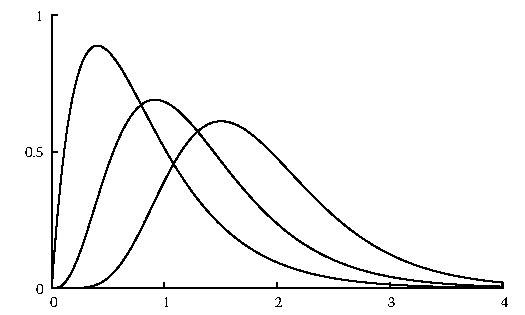
\includegraphics[width=\textwidth]{pdfBetaExp}
\end{center}
\caption[Beta-exponential distributions]{Beta-exponential distributions, (a) $\opr{BetaExp}(x\given 0,1,2, 2)$,
(b) $\opr{BetaExp}(x\given 0, 1, 2, 4)$,
(c) $\opr{BetaExp}(x\given 0, 1, 2, 8)$.
}
\end{figure}

\begin{figure}[p]
\begin{center}
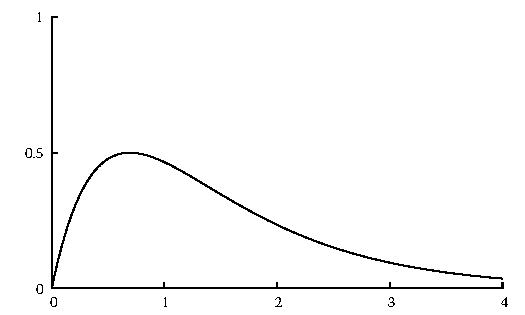
\includegraphics[width=\textwidth]{pdfExpExp}
\end{center}
\caption[Exponentiated exponential distribution]{Exponentiated exponential distribution, $\opr{ExpExp}(x\given 0,1,2)$.
}
\end{figure}


\begin{figure}[ht]
\begin{center}
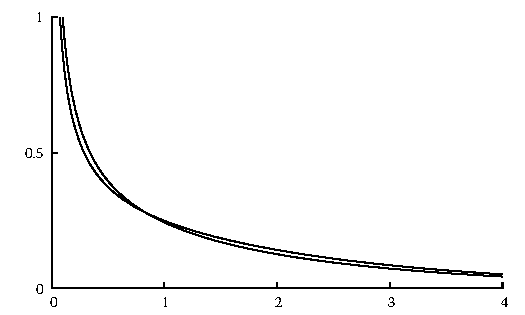
\includegraphics[width=\textwidth]{pdfSinhNK}
\end{center}
\caption[Hyperbolic sine and Nadarajah-Kotz distributions.]{Hyperbolic sine  $\opr{HyperbolicSine}(x\given \tfrac{1}{2})$ and Nadarajah-Kotz $\opr{NadarajahKotz}(x)$ distributions. }
\end{figure}



This distribution has a similar shape to the gamma \eqref{Gamma} distribution. Near the boundary the density scales like $x^{\gamma-1}$, but decays exponentially in the wing.





\SSec{Special cases}

\dist{Exponentiated exponential} (generalized exponential, Verhulst) distribution~\cite{Verhulst1847,Ahuja1967,Gupta2001}:
\begin{align}
\label{ExpExp}
\opr{ExpExp}(x\given \pLoc,\pScale,\gamma) 
 &=  \frac{\gamma}{ \left|\pScale\right|}
 e^{- \frac{x-\pLoc}{\pScale} }  \left(1 - e^{-\frac{x-\pLoc}{\pScale}  }\right)^{\gamma-1} \checked
\\ & = \opr{BetaExp}(x\given \pLoc,\pScale,1, \gamma) \notag \checked
\end{align}
A special case similar in shape to the gamma or Weibull \eqref{Weibull} distribution. So named because the cumulative distribution function is equal to the exponential distribution function raise to a power.
\[
\op{ExpExpCDF}(x\given \pLoc,\pScale,\gamma) = \big[\op{ExpCDF}(x\given \pLoc,\pScale)\big]^{\gamma}
\checked
\notag
\]
% Possibly rename Exponentiated exponential to Verhulst

\begin{table*}[bt]
%\addcontentsline{toc}{subsection}{Logistic} 
\begin{center}
\caption[Beta-exponential distribution -- Special cases]{Special cases of the beta-exponential family}
~\\
{\renewcommand{\arraystretch}{1.25} 
\begin{tabular}{llccccl}
\eqref{BetaExp} & beta-exponential & $\pLoc$ & $\pScale$ & $\alpha$ &  $\gamma$ \\
\hline  
 	& std. beta-exponential & $0$ & $1$ & . & . \\
\eqref{ExpExp} 		& exponentiated exponential & . & . & $1$ & . \\
\eqref{HyperbolicSine} & hyperbolic sine 	& . & .  & $\tfrac{1}{2}(1\text{-}\gamma)$ & $\gamma$ & $0<\gamma<1$ \\
\eqref{NadarajahKotz} &  Nadarajah-Kotz 	& . & . & $\tfrac{1}{2}$ & $\tfrac{1}{2}$ \\
%~\\
%& Related distributions \\
%\hline
\eqref{Exp} & exponential & . & . & . & $1$ \\
%\eqref{GammaExp} & gamma exponential \\ 
\end{tabular} }
\end{center}
\end{table*}


% !TEX encoding = UTF-8 Unicode 
% !TEX root = FieldGuide.tex

\begin{table*}[tp!]
\caption[Beta-exponential distribution -- Properties]{Properties of the beta-exponential distribution}
\begin{align*}
\text{\hyperref[PropertiesSec]{Properties}}  \quad& \\
\text{notation} \quad & \op{BetaExp}(x\given \pLoc,\pScale,\alpha, \gamma)  \checked
\\
\text{PDF}\quad &   \frac{1}{B(\alpha, \gamma)} \frac{1}{|\pScale|} e^{-\alpha \frac{x-\pLoc}{\pScale} }  \left(1 - e^{-\frac{x-\pLoc}{\pScale}  }\right)^{\gamma-1}  \checked
\\
\text{CDF} \big/ \text{CCDF} \quad  & I\left(\alpha,\gamma; e^{-\frac{x-\pLoc}{\pScale}} \right)\checked & \hspace{-2em}\pScale>0 \ \big/ \ \pScale<0
\\
\text{parameters}\quad &   \pLoc,\ \pScale,\ \alpha,\  \gamma \text{ in } \Real	\checked \\
& \alpha,\ \gamma >0	\checked
\\
\text{support} \quad &     x \geq \pLoc \checked&  \pScale > 0
\\
&   x\leq \pLoc  \checked&  \pScale < 0 
\\
%\text{median} \quad  &  \cdots
%\\
%\text{mode} \quad  & \text{not simple}  &\text{\cite{Nadarajah2006}}
%\\
\text{mean} \quad  &  \pLoc+ \pScale [\psi(\alpha+\gamma) -\psi(\alpha)  ]  \checked & \text{\cite{Nadarajah2006}}
\\
\text{variance} \quad  & \pScale^2 [\psi_1(\alpha)-\psi_1(\alpha+\gamma) ]  \checked & \text{\cite{Nadarajah2006}}
\\
\text{skew} \quad  &-\bigl[{\psi_2(\alpha)-\psi_2(\alpha+\gamma)}\bigr] \bigm/ {  \bigl[\psi_1(\alpha)-\psi_1(\alpha+\gamma) \bigr]^{\tfrac{3}{2}} } \checked \hspace{-2em} &  \text{\cite{Nadarajah2006}}
\\
\text{kurtosis} \quad  &
\bigl[3\psi_1(\alpha)^2- 6\psi_1(\alpha)\psi_1(\alpha+\gamma)+ 3\psi_1(\alpha+\gamma)^2+\psi_3(\alpha)
\hspace{-4em} \\ &\qquad -\psi_3(\alpha+\gamma)\bigr] \bigm/ \bigl[ \psi_1(\alpha)-\psi_1(\alpha+\gamma) \bigr]^2
\checked	
 				&  \text{\cite{Nadarajah2006}}
\\
\text{entropy} \quad  & \ln |\pScale| +\ln B(\alpha,\gamma) + (\alpha+\gamma-1) \psi(\alpha+\gamma) 
\\ & \qquad 
- (\gamma -1) \psi(\gamma) - \alpha \psi(\alpha) \checked &\text{\cite{Nadarajah2006}}
\\
\text{MGF} \quad  &e^{\pLoc t }  \frac{B(\alpha-\pScale t, \gamma) }{B(\alpha,\gamma)} \checked & \text{\cite{Nadarajah2006}}
\\                                                                                                                                              
\text{CF} \quad  & e^{i \pLoc t }   \frac{B(\alpha-i \pScale t, \gamma) }{B(\alpha,\gamma)}  \checked & \text{\cite{Nadarajah2006}}
\end{align*}
\end{table*}


\dist{Hyperbolic sine} distribution~\cite{\self}:
\begin{align}
\label{HyperbolicSine}
\opr{HyperbolicSine}(x\given \pLoc, \pScale, \gamma) 
 &=  \frac{1}{ B(\tfrac{1-\gamma}{2}, \gamma)}\frac{1}{|\pScale|}  \bigl( e^{+\frac{x-\pLoc}{2 \pScale}} - e^{-\frac{x-\pLoc}{ 2\pScale}}  \bigr)^{\gamma-1}  
 \checked
\\ \notag  &=  \frac{2^{\gamma-1}}{ B(\frac{1-\gamma}{2}, \gamma) |\pScale| } \bigl(\op{sinh}(\sfrac{x-\pLoc}{2\pScale})\bigr)^{\gamma-1} 
\checked
\\ \notag & = \opr{BetaExp}(x\given \pLoc,\pScale ,\tfrac{1-\gamma}{2}, \gamma), \quad 0<\gamma<1 
\checked
\end{align}
Compare to the hyperbolic secant distribution \eqref{HyperbolicSecant}.

\dist{Nadarajah-Kotz} distribution~\cite{Nadarajah2006,\self} : 
\begin{align}
\label{NadarajahKotz}
\opr{NadarajahKotz}(x\given \pLoc, \pScale) 
 &=  \frac{1}{\pi |\pScale|}  \frac{1}{\sqrt{e^{\frac{x-\pLoc}{\pScale}} -1}}  \checked
\\ \notag & = \opr{BetaExp}(x\given \pLoc,\pScale, \tfrac{1}{2}, \tfrac{1}{2} ) \checked
\end{align}
A notable special case when $\alpha=\gamma=\tfrac{1}{2}$. The cumulative distribution function has the simple form
\[
\op{NadarajahKotzCDF}(x\given 0, 1)= \frac{2}{\pi} \op{arctan} \sqrt{\exp(x) -1} \,  . \checked
\notag
\]
% Self citation is for name of distribution



\SSec{Interrelations}

The  beta-exponential distribution is a limit of the generalized beta distribution \secref{sec:Beta}. The analogous limit of the generalized beta prime distribution \secref{sec:BetaPrime} results in the beta-logistic family of distributions~\secref{sec:BetaLogistic}.


The beta-exponential distribution is the log transform of the beta distribution~\eqref{Beta}.
\[
\oprr{StdBetaExp}{BetaExp}(\alpha,\gamma)  \sim - \ln\bigl( \opr{StdBeta}(\alpha,\gamma) \bigr) 
\checked \notag
\]
It follows that  beta-exponential variates are related to ratios of gamma variates.
\[
\oprr{StdBetaExp}{BetaExp}(\alpha,\gamma)  \sim - \ln  \frac{\opr{StdGamma}_1(\alpha)}{\opr{StdGamma}_1(\alpha)+ \opr{StdGamma}_2(\gamma) }
\checked \notag
\]




The beta-exponential distribution describes the order statistics \secref{OrderStatistic} of the exponential distribution \eqref{Exp}.
\begin{align*}
\opr{OrderStatistic}_{\opr{Exp}(\pLoc,\pScale)} & (x \given  \gamma,\alpha) =  \opr{BetaExp}(x\given \pLoc, \pScale, \alpha, \gamma) \checked
\end{align*}
With  $\gamma=1$ we recover the exponential distribution. 
\[
\opr{BetaExp}(x\given \pLoc, \pScale, \alpha,1) = \opr{Exp}(x\given \pLoc, \tfrac{\pScale}{\alpha})
\checked \notag
\]

The beta-exponential distribution is a limit of the generalized beta distribution~\eqref{GenBeta}, and itself limits to the gamma-exponential distriution~\eqref{GammaExp}.
\[
 \notag
\opr{GammaExp}(x\given \nu, \lambda, \alpha)  & =
{\lim_{\gamma\rightarrow\infty} \opr{BetaExp}(x \given \nu+\lambda/\ln\gamma, \lambda, \alpha, \gamma)  }
\checked \notag
\]





